% DigitaltechnikFS										Stand: 14.01.12
% Digitaltechnik Formelsammlung für SoSe 2011			
% 8 Seiten
% Dokumenteinstellungen
% ======================================================================

% Dokumentklasse (Schriftgröße 6, DIN A4, Artikel)
\documentclass[6pt,a4paper]{scrartcl}

% Seitenlayout und Ränder:
\usepackage{geometry}
\geometry{a4paper,landscape, left=6mm,right=6mm, top=0mm, bottom=3mm,includeheadfoot} 

% Dokumentbeschreibung
\title{Mathe2FSEI SoSe 2011}
\author{Emanuel Regnath, Martin Zellner, Hendrik Böttcher}

% Pakete laden
\usepackage[utf8x]{inputenc}	% Zeichenkodierung: UTF-8 (für Umlaute)   
\usepackage[german]{babel}		% Deutsche Sprache
\usepackage{multicol}			% Spaltenpaket
\usepackage{amsmath}			% Mathematische Formelzeichen
\usepackage{amssymb}			% Mathematische Formelzeichen
\usepackage{esint}				% erweiterte Integralsymbole
\usepackage{multicol}			% ermöglicht Seitenspalten  
\usepackage{booktabs}			% bessere Tabellenlinien
\usepackage{color}				% Farben
\usepackage{colortbl}			% für die Hintergrundfarbe einzelner Zellen in Tabellen
\usepackage{graphicx}			% Grafiken
\usepackage{pbox}				% Intelligent parbox: \pbox{maximum width}{blabalbalb \\ blabal}
%\usepackage{undertilde}			% Tilde unter Zeichen
\newcommand{\utilde}[1]{#1}
\usepackage{scrtime}			% Uhrzeit

%Farben
\definecolor{lightgray}{rgb}{0.8,0.8,0.8}
\definecolor{gray}{rgb}{0.9,0.9,0.9}

% UPDATE WITHOUT CLASS CHANGE
% ----------------------------------------------------------------------

% LastPage
\usepackage{lastpage}

% Allow hyperlinks
	\RequirePackage[pagebackref=true,pdfpagelabels]{hyperref}
	
% Colors
	\RequirePackage{latex4ei/latex4ei_colors}
	\colorlet{col_link}{tum_blue_dark}
	\hypersetup{
	colorlinks=true,
	linkcolor=col_link,
	urlcolor=col_link,
	citecolor=col_link,
}

% set pdfoptions
	\AtBeginDocument{
		\hypersetup{
			pdftitle={Analysis 1},
	        pdfauthor={Lukas Kompatscher},
	        pdfcreator={LaTeX4EI template (www.latex4ei.de)},
	        pdfkeywords={latex4ei}
	    }
	}

% Date with git commit number
	\newcommand{\themydate}{\today} % Default URL placeholder
	\newcommand{\mydate}[1]{\renewcommand{\themydate}{#1}}	

% Header and Footer
	\RequirePackage{fancyhdr}

	\pagestyle{fancy}
	\fancyhf{}

	\AtBeginDocument{
	\IfFileExists{git.id}{\input{git.id}}{}
	\ifdefined\GitNiceDate\mydate{\GitNiceDate\ (git \GitRevision)}\fi
	\ifdefined\GitIssuesURL
		\ifdefined\setissueslinkurl
		\setissueslinkurl{\GitIssuesURL} % Set the actual URL
		\fi
	\fi
	}
	
% Define Email
	\providecommand{\email}[1]{\href{mailto:#1}{\nolinkurl{#1}}}
	
%
	\fancyfoot[C]{von Lukas Kompatscher\ -- Mail: \email{lukas.kompatscher@tum.de}}
	\fancyfoot[R]{Stand: \themydate \qquad \thepage/\pageref{LastPage}}
	\fancyfoot[L]{Homepage: \url{www.latex4ei.de} -- Fehler bitte \emph{sofort} \href{\issueslinkurl}{melden}.}
	
	\renewcommand{\headrulewidth}{0.0pt} %obere Linie ausblenden
	\renewcommand{\footrulewidth}{0.1pt} %obere Linie ausblenden
	
	\newcommand{\issueslinkurl}{https://github.com/latex4ei/Allgemein/issues} % Default URL placeholder
	\newcommand{\setissueslinkurl}[1]{\renewcommand{\issueslinkurl}{#1}}
% ----------------------------------------------------------------------
	
% Schriftart SANS für bessere Lesbarkeit bei kleiner Schrift
\renewcommand{\familydefault}{\sfdefault} 
\renewcommand{\emph}[1]{\textsf{\textbf{#1}}}

% Array- und Tabellenabstände vergrößern
\renewcommand{\arraystretch}{1.2}
\renewcommand{\vec}[1]{\ensuremath{\underline{\boldsymbol {#1}}}}


% Eigene Befehle
\newcommand{\todayV}{\the\day.\the\month.\the\year}                     	    	% Datum D.M.YYYY
\newcommand{\iset}[2]{\ensuremath{\bigl\{ \bigl. #1 \, \bigr| \, #2 \bigr\}}}		% intensional set
\newcommand{\eset}[1]{\ensuremath{\bigl\{#1\bigr\}}}								% extensional set
\newcommand{\norm}[1]{\ensuremath{\|#1\|}}											% Norm
\newcommand{\gk}[1]{\ensuremath{\left\lfloor#1\right\rfloor}} 						% Gaußklammer
\newcommand{\sprod}[2]{\ensuremath{\left\langle #1, #2 \right\rangle }}				% Skalarprodukt
\newcommand{\abs}[1]{\ensuremath{\left\vert#1\right\vert}} 							% Betrag
\newcommand{\mat}[1]{\ensuremath{\begin{bmatrix} #1 \end{bmatrix}}}					% Matrix
\newcommand{\vect}[1]{\ensuremath{\begin{pmatrix} #1 \end{pmatrix}}}				% Vektor
\newcommand{\mvect}[1]{\ensuremath{\left. \begin{matrix} #1 \end{matrix}  \right]}} % Matrixvektor
\newcommand{\ma}[1]{\ensuremath{\utilde{\bs {#1}}}}

% Abkürzungen
\newcommand{\ul}[1]{\ensuremath{\underline{#1}}}								%Untersteichen
\newcommand{\ol}[1]{\ensuremath{\overline{#1}}}									%Überstreichen
\newcommand{\Ra}[0]{\ensuremath{\Rightarrow}}									%Rightarrow
\newcommand{\ra}[0]{\ensuremath{\rightarrow}} 									%Rightarrow
\newcommand{\n}[0]{\ensuremath{\overline}}										%NOT
\newcommand{\bs}[1]{\ensuremath{\boldsymbol{#1}}}								%Fett und kursiv im mathmode
\newcommand{\diff}{\ensuremath{\ \mathrm d}}									%delta
\newcommand{\grad}{\ensuremath{\mathrm{grad}\ }}								%Gradient
\renewcommand{\div}{\ensuremath{\mathrm{div}\ }}								%Divergenz
\newcommand{\rot}{\ensuremath{\mathrm{rot}\ }}									%Rotation
\newcommand{\Sp}{\ensuremath{\mathrm{Sp}\ }}									%Spur
	% Für Mengen
	\newcommand{\N}{\ensuremath{\mathbb N}}
	\newcommand{\R}{\ensuremath{\mathbb R}}
	\newcommand{\C}{\ensuremath{\mathbb C}}

%Überschreibungen
\renewcommand{\arraystretch}{1.2}
\renewcommand{\vec}[1]{\ensuremath{\underline{\boldsymbol {#1}}}}


% Dokumentbeginn
% ======================================================================

\begin{document}


% Aufteilung in Spalten
\begin{multicols}{3}

% -------------------------------------------
% | 		Digitaltechik					|
% ~~~~~~~~~~~~~~~~~~~~~~~~~~~~~~~~~~~~~~~~~~~
%=======================================================================
\parbox{2.3cm}{
	
\includegraphics[height=2cm]{img/Logo.pdf}
}
\parbox{4cm}{
	\emph{\huge{Digitale Schaltungen}}
}

% ======================================================================
\section{Moore'sches Gesetz}
\begin{itemize} \itemsep0pt
	\item alle 18-24 Monate verdoppelt sich die Anzahl der Transistoren auf gleicher Fläche
	\item Exponentielles Wachstum der Transistorzahl, exponentieller Rückgange des Preises pro Transistor
	\item Herstellungskosten (Fixkosten, Variable Kosten, Technologiefaktor), Entwicklerproduktivität, Verlustleistungsdichte
\end{itemize}

\section{Einheiten}
\begin{multicols}{3}
\begin{tabular}{c | c}
	Potenz & Vorsatz \\ \midrule
	$10^{12}$ & T \\
	$10^{9}$ & G \\
	$10^{6}$ & M \\
	$10^{3}$ & k \\
	$10^{2}$ & h \\
	$10^{1}$ & da 
\end{tabular}
\begin{tabular}{c | c}
	Potenz & Vorsatz \\ \midrule
	$10^{-1}$ & d \\
	$10^{-2}$ & c \\
	$10^{-3}$ & m \\
	$10^{-6}$ & $\mu$	\\
	$10^{-9}$ & n \\
	$10^{-12}$ & p \\
	$10^{-15}$ & f
\end{tabular}
\begin{tabular}{ r | l }
$Hz$ & $s^{-1}$ \\
N & $kg m s^{-2} $ \\
$J $ & $ N m = V A s$\\
$W $ & $ V A  = J s^{-1} $ \\
$ C $ & $ A s $ \\
$V $ & $ J C^{-1} $\\
$F $ & $ C V^{-1} $ \\
$\Omega $ & $ V A^{-1} $\\
$ H $ & $ V s  A^{-1}$
\end{tabular}
\end{multicols}
$Bit \xrightarrow{\cdot 8} Byte \xrightarrow{\cdot 1024} kByte \xrightarrow{\cdot 1024} MByte$\\

\section{Polyadische Zahlensysteme}
$Z = \sum\limits^{p-1}_{i = -n} r^i \cdot d_i = d_{p-1}...d_1 d_0 . d_{-1} ... d_n$\\
$Z$:Zahl, \ \ $r$:Basis, \ \ $d_i$:Ziffer, \ \ $p$:\#Ziffern vorne \ \ $n$:\#Nachkommastellen

Binäres Zahlensystem:\\
$d_{i2} \in {0,1}$ \qquad
$B = \sum\limits_{i=-n}^{p-1} 2^i \cdot d_i$ $\quad d_{-n}: LSB; \quad d_{p-1}: MSB$ \\
\begin{tabular}{l|l}
Octalsystem: & Hexadezimalsystem:\\
$d_{i8} \in {0,1,2,3,4,5,6,7}$ & $d_{i16} \in {0,1,2,3,4,5,6,7,8,9,A,B,C,D,E,F}$\\
\end{tabular}\\
\\

Benötigte Bits: $N: n$ Bit  $M: 2n$ Bit \\
$N + M = 2n +1$ Bit \\
$N \cdot M = 3n$ Bit
	\subsection{Umrechnung}
	\begin{tabular}{l|l|l}
			& $Z \ge 1$ & $Z < 1$\\ \midrule
		$r \rightarrow 10$ & $Z_{10} = \sum r^i \cdot d_i$ & $Z_{10} = \sum r^{-i} \cdot d_{-i}$\\
		& $101_2 \ra 1 \cdot 1 + 0\cdot 2 + 1 \cdot 4$ & $0.11_2 \ra 1\cdot 0.5 + 1\cdot 0.25$\\ \midrule
		$10 \rightarrow r$ & $d_i = Z_{10} \% r^i$ & \\
		& $58 / 8 = 7\text{Rest}\ 2 (LSB)$ & $0.4 \cdot 2 = 0.8 \text{ Übertrag } 0 (MSB)$\\
		& $7 / 8 = 0\text{ Rest } 7 (MSB)$ & $0.8 \cdot 2 = 1.6 \text{ Übertrag } 1$ \\
	\end{tabular}

	\subsection{Zweierkomplement \qquad Wertebereich: $-2^{n-1} \le Z \le 2^{n-1} -1$}
	Wandle 2 in -2 um:\\
		\begin{tabular}{l|l}
			1. Invertieren aller Bits  & $0010 \ \Rightarrow 1101$\\
			2. Addition von 1	& $1101 + 1 = 1110$\\
			3. Ignoriere Überträge beim MSB & $\Rightarrow \ -2_{10} = 1110_2$\\
		\end{tabular}
	\subsection{Gleitkommadarstellung nach IEEE 754}
	\begin{tabular}{l|l}
		$Wert = (-1)^s \cdot 2^{e-127} \cdot 1.f$ & Bsp: $-0.625 = -1 \cdot 2^{-1} \cdot 1.01_2$\\
		$s$: Vorzeichen, $e$: Exponent, $f$: Mantisse & $\Ra\ s = 1$, $e = 126$, $f = 01_2$\\ 
	\end{tabular}
	\\[0.5em]
	Spezialwerte: $Wert = 0 \Leftrightarrow e=0$ \qquad $Wert = \infty \Leftrightarrow e=255$ \\
	Bitverteilung(single/double):\\
	\begin{tabular}{|c|c|c|} \hline 
		$s(1)$ & \quad $e(8/11)$ \quad\qquad & \qquad\qquad\qquad\ $f(23/52)$ \qquad\qquad\qquad\qquad \\ \hline
	\end{tabular}

\section{Halbleiter}
\begin{tabular}{l|c|c|c|c|c}
	& Isolator & Metall & undotiert & N-Typ & P-Typ \\ \hline
	Ladungsträger & Keine & $e^-$ & $e^- / e^+$ & $e^-$ & $e^+$ \\
	Leitfähigkeit & Keine & Sehr hoch & $\propto T$ & Hoch & Mittel\\  
\end{tabular}


\section{MOS-FET's}
% ======================================================================
\textbf{M}etal \textbf{O}xide \textbf{S}emiconductor \textbf{F}ield \textbf{E}ffekt \textbf{T}ransistor\\
\parbox{4.0cm}{ 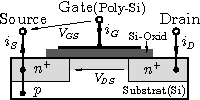
\includegraphics{img/ds/mosfet.pdf} \\ $V_{Pinch-Off} = V_{GS} - V_{th}$ } \parbox{3.0cm}{ 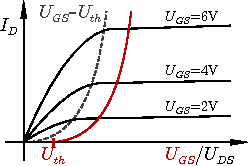
\includegraphics{img/ds/char_nmos.pdf} } 


	\subsection{Bauteilparameter}
	Verstärkung: \framebox{
			$\beta = K' \frac{W}{L} \text{ mit } K' = \frac{\mu \epsilon_{0x} \epsilon_0}{t_{0x}} $
		} \\
	\begin{tabular} {r | l}
		Kanalweite & W  \\
		Kanallänge & L  \\
		Elektronenbeweglichkeit & $\mu$\quad $\mu_n \approx 250 \cdot 10^{-4} \frac{m^2}{Vs}$, $\mu_p \approx 100 \cdot 10^{-4} \frac{m^2}{Vs}$ \\
		rel. Dielektrizität des Gateoxyds & $\epsilon_{ox} \approx 3,9$ \\
		Dielektrizitätskonstante & $\epsilon_0 = 8.8541878 \cdot 10^{-12} \frac{\mathrm{A\,s}}{\mathrm{V\,m}}$ \\
		Gateoxyddicke & $t_{ox}$ \\
		Verstärkung & $\beta = \frac{\mu_n \varepsilon_{ox} \varepsilon_0}{t_{ox}} \cdot \frac{W}{L} = K' \frac{W}{L} = \frac{\mu_n C_G}{L^2}$ \\
		Kapazität & $C_G = \varepsilon_{ox} \varepsilon_0 \frac{WL}{t_{ox}}$ \\
		Verzögerungszeit & $t_{pHL} \propto \frac{C_L t_{ox} L_p}{W_p \mu_p \varepsilon_{ox} (V_{DD} - |V_{th}|)}$ \\
	\end{tabular}
	\begin{itemize}
		\item große Kanalweite $\Ra$ große Drain-Störme \\ $\Ra$ schnelle Schaltgeschwindigkeit (da $i_d \propto \beta \propto \frac{W}{L}$) \\
		Aber: große Fläche.
		\item nMos schaltet schneller als pMOS 
	\end{itemize}
	
	
	\subsection{pMos und nMos}
	\pbox{3.0cm}{ 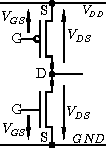
\includegraphics{img/ds/cmos.pdf} } 
	\pbox{10.0cm}{
	\begin{tabular}{c|c|c|c}
		Transistor & Source liegt immer am & $V_{GS},V_{DS},I_D$ & Substrat \\ \midrule
		$\underset{\text{normally on}}{\text{pMos}}$ & höheren Potential & $\bs{< 0}$ & $+(V_{DD})$ \\
		& & & \\
		& & & \\
		$\underset{\text{normally off}}{\text{nMos}}$ & niedrigeren Potential & $\bs{> 0}$ & $-(GND)$ \\
	\end{tabular}\\[0.5cm]
	}\\	
	
	Drainstromformel:\\
	nMos (p-dotiertes Substrat, n-dotierte Drain/Source), schlechter pull up (Pegeldegenerierung)
	\begin{equation*}
	\!\!\! I_d = \begin{cases}
	0, &\text{ für }  U_{gs} - U_{th} \le 0 \qquad \qquad  \text{(Sperrber.)}\\[0.2em]
	 \beta [(u_{gs} - U_{th}) \cdot u_{ds} - \frac{1}{2} u_{ds}^2] , &\text{ für }  0 \le U_{gs} - U_{th} \ge u_{ds} \  \text{(linearer Ber.)}\\\\[0.2em]
	 \frac{1}{2} \beta \cdot (u_{gs} - U_{th})^2, &\text{ für }  0 \le U_{gs} - U_{th} \le u_{ds} \  \text{(Sättigungsber.)}\\

	\end{cases}
	\end{equation*}
	Drainstromformel: \\
	pMos (n-dotiertes Substrat, p-dotierte Drain/Source), schlechter pull down (Pegeldegenerierung)
	\begin{equation*}
	\!\!\! I_d = \begin{cases}
	0, &\text{ für }  U_{gs} - U_{th} \ge 0 \qquad \qquad  \text{(Sperrber.)}\\[0.2em]
	- \beta [(u_{gs} - U_{th}) \cdot u_{ds} - \frac{1}{2} u_{ds}^2] , &\text{ für }  0 \ge U_{gs} - U_{th} \le u_{ds} \  \text{(linearer Ber.)}\\\\[0.2em]
	- \frac{1}{2} \beta \cdot (u_{gs} - U_{th})^2, &\text{ für }  0 \ge U_{gs} - U_{th} \ge u_{ds} \  \text{(Sättigungsber.)}\\

	\end{cases}
	\end{equation*}



\subsection{Disjunktive Normalform (DNF/SOP)}
Eins-Zeilen der Wertetabelle ODER verknüpfen: \\
$Z = \overline A \cdot \overline B + \overline C \cdot D$

\subsection{Konjunktive Normalform (KNF/POS)}
Null-Zeilen der Wertetabelle negieren und UND verknüpfen: \\	
$Z = ( \ol A + \ol C) \cdot ( \ol A + \ol D) \cdot ( \ol B + \ol C) \cdot ( \ol B + D)$

\subsection{Umwandlung in jeweils andere Form}
1. Doppeltes Negieren der Funktion: $ Z = \overline {\overline{\overline A \cdot \overline B + \overline C \cdot D}}$\\
2. Umformung "'untere"'  Negation (DeMorgan) : $ Z = \ol{\ol{\ol A \cdot \ol B} \cdot \ol{\ol C \cdot D}} = \ol{(A+B) \cdot (C+\ol D)}$\\
3. Ausmultiplizieren: $ Z = \ol{(A+B) \cdot (C+\ol D)} = \ol{A\cdot C + A\cdot \ol D + B \cdot C + B \cdot \ol D}$\\
4. Umformung "'obere"'  Negation (DeMorgan) :\\ $ Z= \ol{AC} \cdot \ol{A \ol D} \cdot \ol{BC} \cdot \ol{B\ol D} = ( \ol A + \ol C) \cdot ( \ol A + D) \cdot ( \ol B + \ol C) \cdot ( \ol B + D)$\\
Analog von KNF nach DNF.
\section{CMOS - Logik}
% ======================================================================
Komplementäre Logik liefert grundsätzlich negierte Ausgänge. $\Rightarrow$ NAND einfacher als AND.\\
Drei Grundgatter der CMOS-Technologie:\\
	\begin{tabular}{ccc}
		NOT (2 Trans.) & NAND (4 Trans.) & NOR (4 Trans.)\\
		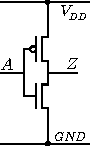
\includegraphics{img/ds/mosfet_not.pdf} \quad & 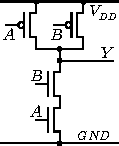
\includegraphics{img/ds/mosfet_nand.pdf} \quad & 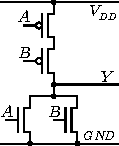
\includegraphics{img/ds/mosfet_nor.pdf} \\
	\end{tabular}\\
	Falls $GND$ und $V_{DD}$ vertauscht würden, dann $NAND \ra AND$ und $NOR \ra OR$\\
	Allerdings schlechte Pegelgenerierung.
	
	\subsection{Gatterdesign}
	\emph{Vorteil:}	 (Fast) nur bei Schaltvorgängen Verlustleistung - wenig statische Verluste
	\begin{tabular}{l|l|l}
		Netzwerk & Pull-Dow\bf{n} & Pull-U\bf{p} \\ \midrule
		Transistoren & \textbf{n}Mos & \textbf{p}Mos \\
		AND & Serienschaltung	 & Parallelschaltung \\
		OR & Parallelschaltung & Serienschaltung \\
	\end{tabular}\\
	1. Möglichkeit: Direkt; ggf. Inverter vor die Eingänge und Ausgänge schalten.\\
	2. Möglichkeit: Mit bullshit Algebra die Funktion nur mit NAND und NOR darstellen.\\

	\subsection{CMOS Verlustleistung}
	Inverterschaltvorgang $V_A: 0 \ra 1$:\\
	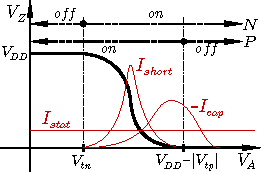
\includegraphics{img/ds/char_inverter.pdf}
	
	\begin{tabular}{ll}
		\emph{Dynamische Verlustleistung}	& $P_{dyn} = P_{cap} + P_{short}$\\
		\quad Kapazitive Verluste & $P_{cap} = \alpha_{01} f C_L V_{DD}^2$\\
		\quad Kurzschlussstrom	& $P_{short} = \alpha_{01} f \beta_n \tau (V_{DD} - 2V_{tn})^3$\\[0.8em]
		\quad Schalthäufigkeit & $\alpha_{0 \rightarrow 1} = \frac{\text{Schaltvorgänge(pos. Flanke)}}{\text{\# Betrachtete Takte}}$\\
	\end{tabular}\\
	
	Abhängig von den Signalflanken, mit Schaltfunktionen verknüpft\\ 
	$\approx \;$ $V_{DD} 1/\propto $ Schaltzeit: $\frac{V_{DD2}}{V_{DD1}} = \frac{t_{D1}}{t_{D2}}$ (bei Schaltnetzen $t_{log}$)\\
	Verzögerungszeit $\propto$ $\frac{1}{V_{DD} - V_{th}}$\\

	\emph{Statische Verlustleistung} $P_{stat}$: Sub-Schwellströme, Leckströme, Gate-Ströme
	
	Abhängigkeit: $V_{DD}\uparrow:P_{stat}\uparrow$ \qquad $V_{th}\uparrow:P_{stat}\downarrow$ \quad (aber nicht proportional)\\


\section{Sequentielle Logik}
... Logik mit Gedächtnis. Bedingungen: \\
\begin{tabular}{c | l}
$t_{Setup}$ & Stabilitätszeit vor der aktiven Taktflanke\\
$t_{hold}$ & Stabilitätszeit nach  der aktiven Taktflanke\\
$t_{c2q}$ & Eingang wird spätestens nach $t_{c2q}$ am Ausgang verfügbar\\
Max. Taktperiode &  $t_{clk} \ge t_{1,c2q} + t_{logic,max} + t_{2,setup}$  \\
 Max. Taktfrequenz & $f_{max} = \left\lfloor \frac{1}{t_{clk}} \right\rfloor$ \qquad (Nicht aufrunden) \\
 Holdzeitbedingung & $t_{hold} \le t_{c2q} + t_{logic,min}$  $\ra$ Dummy Gatter einbauen\\
 Durchsatz & $\frac{1 \text{Sample}}{t_{clk,pipe}} = f$ \\
 Latenz & $t_{clk} \cdot \#$Pipelinestufen (das zwischen den FFs) \\
\end{tabular}


\subsection{Pipelining} % (fold)
Nur bei synchronen(taktgesteuerten) Schaltungen möglich!
\begin{itemize} \itemsep0pt
	\item Aufteilen langer kombinatorischer Pfade durch Einfügen zusätzlicher Registerstufen\\
	$\ra$ Möglichst Halbierung des längsten Pfades
	\item Zeitverhalten beachten (evtl. Dummy-Gatter einfügen)
	\item Durchsatz erhöht sich entsprechend der Steigerung der Taktfrequenz
	\item Gesamtlatenz wird eher größer
	\item Taktfrequenz erhöht sich
\end{itemize}
% subsection Pipelining (end)

\subsection{Parallel Processing} % (fold)

Durchsatz = $\frac{\#\text{Modul}}{t_{clk,Modul}} = f$ \qquad \quad Latenz = $t_{clk}$
\begin{itemize} \itemsep0pt
	\item Paralleles, gleichzeitiges Verwenden mehrere identischer Schaltnetze
	\item Zusätzliche Kontrolllogik nötig (Multiplexer)
	\item Taktfrequenz und Latenz bleiben konstant
	\item Durchsatz steigt mit der Zahl der Verarbeitungseinheiten \\
	ABER: deutlich höherer Ressourcenverbrauch
\end{itemize}
% subsection Parallel Processing (end)

\section{Volladdierer (VA) / Ripple-C(u)arry-Adder}
\parbox{5.0cm}{ 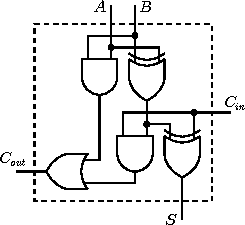
\includegraphics{img/ds/volladdierer.pdf} }
\pbox{6.0cm}{
Generate $g_n = a_n \cdot b_n$\\
Propagate $p_n = a_n \oplus b_n$\\
Summenbit $S_n = c_n \oplus p_n$\\
Carry-out: $c_{n+1} = c_n \cdot p_n + g_n$\\ \\
Laufzeiten: \\
$t_{sn} = \begin{cases} t_{cn} + t_{xor} & t_{cn} > t_{xor} \\ 2 t_{xor} & sonst \end{cases}$\\ }\\
$t_{cn+1} = \begin{cases} t_{and} + t_{or} & p_n = 0, g_n=1 \\ t_{xor} + t_{and} + t_{or} & p_n = 0, g_n = 0 \\ t_{cn} + t_{and} + t_{or} & p_n = 1 \end{cases}$\\




\section{Speicherelemente}
	\emph{Flüchtig} Speicherinhalt gehen verloren, wenn Versorgungsspannung $V_{DD}$ wegfällt - Bsp: *RAM\\
	\emph{Nicht Flüchtig} Speicherinhalt bleibt auch ohne $V_{DD}$ erhalten - Bsp: Flash\\
	\emph{Asynchron} Daten werden sofort geschrieben/gelesen.\\
	\emph{Synchron} Daten werden erst mit $clk_{0 \ra 1}$ geschrieben.\\
	\emph{Dynamisch} Ohne Refreshzyklen gehen auch bei angelegter $V_{DD}$ Daten verloren -  Bsp: DRAM\\
	\emph{Statisch} Behält den Zustand bei solange $V_{DD}$ anliegt (keine Refreshzyklen nötig) - Bsp: SRAM\\
	\begin{description}
		\item[Bandbreite:] Bitanzahl, die gleichzeitig gelesen/geschrieben werden kann.
		\item[Latenz:] Zeitverzögerung zwischen Anforderung und Ausgabe von Daten.
		\item[Zykluszeit:] Minimale Zeitdifferenz zweier Schreib/Lesezugriffe.
	\end{description}
	
	\framebox{$\text{Speicherkapazität} = \text{Wortbreite} \cdot 2^\text{Adressbreite}$ }

	\subsection{Flip-Flop}
	\begin{multicols}{2}
	besteht aus zwei enable-Latches \\
	\emph{Flip-Flop:} ändert Zustand bei steigender / (fallender) Taktflanke.\\
	\begin{tabular}{c|c|c} $clk$ & $Q$ & $\ol Q$ \\ \hline $0 \ra 1$ & $D$ & $\ol D$ \\ sonst & $Q$ & $\ol Q$ \end{tabular}
	\end{multicols}
	\subsection{Register}
	Ring aus zwei Invertern.

	\subsection{Latch}
	\begin{multicols}{2}
	\emph{Set-Reset Latch:} \\ Zwei gegenseitig rückgekoppelte NAND-Gatter. $0$ an R/S schaltet. \\
	\emph{Enable-Latch:} ändert Speicherzustand auf $D$ nur wenn $e=1$: \begin{tabular}{c|c} e & Q \\ \hline 0 & Q \\ 1 & D \end{tabular}
	\end{multicols}
	\subsection{DRAM Zelle (dynamisch)}

	\parbox{3.0cm}{ 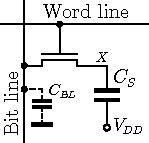
\includegraphics{img/ds/DRAM.pdf} }
	\parbox{6.0cm}{ 
	
	lange Bitlines $\ra C_{BL} \uparrow$, Laufzeit$\uparrow$\\
	quadratisch: $\frac{\text{Bit}}{\text{Zeile}} \stackrel{!}= \frac{\text{Bit}}{\text{Spalte}} = \frac{\text{Wort}}{\text{Zeile}} \cdot \frac{\text{Bit}}{\text{Wort}}$\\
	
	\paragraph{Schreiben}
		\begin{itemize}\itemsep0pt
			\item Wortleitung wird aktiviert, d.h. auf $V_{DD}$ gelegt
			\item Bitleitung wird auf den gewünschten Wert ($V_{DD}$ für $1$, GND für $0$) gelegt \\
			$\Ra$ Kondensator wird auf entsprechendes Potential aufgeladen oder entladen, je nach vorherigem Wert
		\end{itemize}
	}
	
	\paragraph{Lesen}
	\begin{itemize}\itemsep0pt
		\item Wortleitung wird aktiviert, d.h. auf $V_{DD}$ gelegt. 
		\item Bitleitung wird auf $V_{DD} / 2$ vorgeladen.
		\item Adresstransistor wird geöffnet \\
		$\ra$ Ladungsaustausch zwischen $C_S$ und $C_{BL}$ \\
		$\ra$ Potential der BL wird um $\Delta V$ erhöht ($1$ lesen) oder erniedrigt ($0$ lesen) \\\
		$\ra$ $\Delta V = \left(V_X - \frac{V_{DD}}{2}\right) \cdot \frac{C_S}{C_S + C_{BL}}$ \quad i.d.R $C_{BL} >> C_S \ra \Delta V$ sehr klein \\
		$\ra $ Leseverstärker nötig!
	\end{itemize}

\begin{multicols}{2}	
	\subsection{SRAM Zelle (statisch)}
	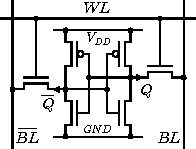
\includegraphics{img/ds/SRAM.pdf}


	\subsection{ROM - Read Only Memory}
	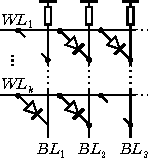
\includegraphics{img/ds/ROM.pdf}
\end{multicols}

	\subsection{Flash (nicht flüchtig)}
	nMos Transistor mit zusätzlichem floating Gate in der Oxidschicht.\\
	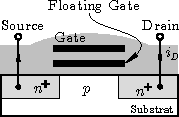
\includegraphics{img/ds/flash.pdf} \qquad 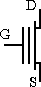
\includegraphics{img/ds/flashsymbol.pdf}\\
	‚0’ speichern: $V_{GS} = V_{DS} = 4 \cdot V_{DD}$, S an GND\\
	‚0’ löschen: S von GND trennen, G an GND und D an 4mal VDD\\
 

\subsection{Organisation von Speichern} 

\begin{itemize} \itemsep0pt
	\item 1 Byte besteht aus 8 Bit
	\item Ziel: möglichst quadratische Anordnung der Speicherzellen
	\item Wortbreite W berücksichtigen!	
\end{itemize}
Aufteilung:\\
Speicherkapazität $= 2^M \cdot 2^N$ Bester Fall für $M=N$\\ 
\# Reihen $= N$\\
$2^M = W \cdot 2^K$\\
\# Spalten $= K$\\









\section{Automaten} % (fold)

DFA 6-Tupel $\eset{I, O, S, R, f, g}$ \\

\begin{tabular}{r | l} 
$I$ & Eingabealphabet \\
$O$ &  Ausgabealphabet \\
$S$ & Menge von Zuständen \\
$R \subseteq S$ &  Menge der Anfangszustände \\
$f: S \times I \ra S$  &  Übergangsrelation \\
$g$ & Ausgaberelation \\
\end{tabular}

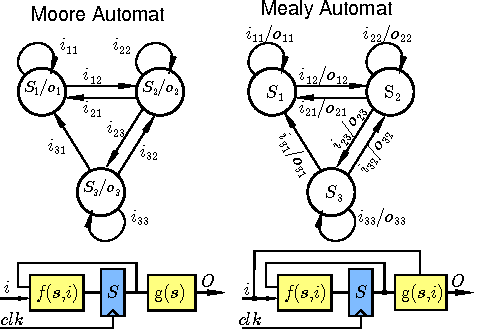
\includegraphics{img/ds/automaten.pdf}\\


\begin{tabular}{c | c}
 Moore & Mealy \\ \midrule
 Ouput hängt nur vom Zustand ab & Output hängt von Zustand und Eingabe ab\\
 $g: S \ra O$ & $g: S \times I \ra O$
\end{tabular}

\subsection{Vorgehensweise} % (fold)
\begin{itemize}
	\item $I, O$ bestimmen
	\item $S$ festlegen 
	\item $R$ bestimmen
	\item $f,g$ bestimmen
\end{itemize}
% subsection Vorgehensweise (end)

% Ende der Spalten
\end{multicols}









































\newpage
\begin{multicols}{3}
% -----------------------------------------------
% | 	E N T W U R F S V E R V A H R E N		|
% ~~~~~~~~~~~~~~~~~~~~~~~~~~~~~~~~~~~~~~~~~~~~~~~
%=======================================================================

\parbox{2.3cm}{
	
\includegraphics[height=2cm]{img/Logo.pdf}
}
\parbox{4cm}{
	\emph{\huge{Entwurfsverfahren}}
}

\setcounter{section}{0}			% Zähler für Sections zurücksetzen

\section{Boolsche Algebra}
	\begin{tabular}{l|l|l}
		& Mengenalgebra & Boolesche Algebra \\ 
		& $(P(G);\cap , \cup, \overline{A};G,\emptyset )$ & $({0,1};\cdot , +, \overline{x})$ \\ \midrule
		Kommutativ 		& $A \cap B = B \cap A$ & $x \cdot y = y \cdot x$  \\ 
						& $A \cup B = B \cup A$ & $x + y = y + x$\\
		Assoziativ 		& $(A \cap B) \cap C = A \cap (B \cap C)$ & $x \cdot (y \cdot z) = (x \cdot y) \cdot z$\\
						& $(A \cup B) \cup C = A \cap (B \cup C)$ & $x + (y + z) = (x + y) + z$\\
		Distributiv 	& $A \cap (B \cup C) = (A \cap B) \cup (A \cap C)$ & $x \cdot (y + z) = x \cdot y + x \cdot z$\\
						& $A \cup (B \cap C) = (A \cup B) \cap (A \cup C)$ & $x + (y \cdot z) = (x + y) \cdot (x + z)$\\
		Indempotenz		& $A \cap A = A$ & $x \cdot x = x$ \\
						& $A \cup A = A$ & $x + x = x$\\
		Absorbtion		& $A \cap (A \cup B) = A$ & $x \cdot (x+y) = x$ \\
						& $A \cup (A \cap B) = A$ & $x + (x \cdot y) = x$ \\
		Neutral			& $A \cap G = A$ & $x \cdot 1 = x$ \\
						& $A \cup \emptyset = A$ & $x + 0 = x$ \\
		Dominant		& $A \cap \emptyset = \emptyset$ & $x \cdot 0 = 0$ \\
						& $A \cup G = G$ & $x + 1 = 1$ \\
		Komplement		& $A \cap \overline{A} = \emptyset$ & $x \cdot \overline{x} = 0$\\
						& $A \cup \overline{A} = G$ & $x + \overline{x} = 1$\\
						& $\overline{\overline{A}} = A$ & $\overline{\overline{x}} = x$\\
		De Morgan		& $\overline{A \cap B} = \overline{A} \cup \overline{B}$ & $\overline{x \cdot y} = \overline{x} + \overline{y}$\\
						& $\overline{A \cup B} = \overline{A} \cap \overline{B}$ & $\overline{x + y} = \overline{x} \cdot \overline{y}$\\

	\end{tabular}
	\\
	
	
	\subsection{Multiplexer}
	\begin{tabular}{ll}
		$f = x \cdot a + \overline x \cdot b$ & (2 Eingänge $a,b$ und 1 Steuereingang $x$)\\
		$f = \ol x_1 \ol x_2 a + \ol x_1 x_2 b + x_1  \ol x_2 c + x_1 x_2d$ & (Eingänge: $a,b,c,d$  Steuerung: $x_1$, $x_2$)\\
	\end{tabular}



	\subsection{Wichtige Begriffe}
	\begin{tabular}{l|l|l}
		Wichtige Begriffe: & Definition & Bemerkung\\ \hline
		Signalvariable & $x$ & $\hat x \in \eset{0,1}$ \\
		Literal & $l_i = x_i$ oder $\overline{x_i}$ & $i \in I_0=\eset{1,...,n}$\\
		Minterme,0-Kuben & M0C $\ni m_j = \prod\limits_{i\in I_0} l_i$ & $|$M0C$| = 2^n$ \\
		d-Kuben & MC $\ni c_j = \prod\limits_{i\in I_j \subseteq I_0} l_i$ & $|$MC$|=3^n$\\
		Distanz & $\delta(c_i,c_j) = \bigl| \iset{l}{l \in c_i \land \overline{l}\in c_j}  \bigr|$ & $\delta_{ij} = \delta(c_i,c_j)$ \\
		Implikanten & $MI = \iset{c \in MC}{c \subseteq f}$ &  \\
		Primimplikanten & $MPI = \iset{p \in MI}{p \not\subset c \ \forall c \in MI}$ & $MPI \subseteq MI \subseteq MC$\\
	\end{tabular}\\ \\ \\
	\begin{tabular}{l|l|l}	
		SOP (DNF) & eine Summe von Produkttermen & Terme sind ODER-verknüpft \\
		POS (KNF) & ein Produkt von Summentermen & Terme sind UND-verknüpft\\
		CSOP (nur 1)& Menge aller Minterme & analog CPOS \\
		VollSOP (nur 1)& Menge aller Primimplikanten & Bestimmung siehe Quine Methode\\
		& & oder Schichtenalgorithmus\\
		MinSOP (min. 1)& Minimale Summe v. Primimplikanten & durch Überdeckungstabelle \\
	\end{tabular}
	\\ \\
	FPGA: Field Programmable Gate Array\\
	LUT: Look Up Table\\


	\subsection{Boolesche Operatoren (Wahrheitstabelle WT)}
	\begin{tabular}{c|c||c|c|c|c|c|c}
		x & y & AND & OR & XOR & NAND & NOR & EQV \\ 
		& & $x\cdot y$ & $x+y$ & $x\oplus y$ & $\overline{x\cdot y}$ & $\overline{x+y}$ & $\overline{x\oplus y}$ \\ \hline \hline
		0 & 0 & 0 & 0 & 0 & 1 & 1 & 1  \\ \hline
		0 & 1 & 0 & 1 & 1 & 1 & 0 & 0 \\ \hline
		1 & 0 & 0 & 1 & 1 & 1 & 0 & 0 \\ \hline
		1 & 1 & 1 & 1 & 0 & 0 & 0 & 1 \\
	\end{tabular}

Konfiguration: $f = c_1 + c_2 + c_3 \Ra cov(f) = \eset{c_1, c_2, c_3}$



\section{Beschreibungsformen}

\subsection{Sum of products (SOP/DNF)}
Eins-Zeilen der Wertetabelle ODER verknüpfen: \\
$f = \overline x \cdot \overline y + \overline z \cdot w$

\subsection{Product of sums (POS/KNF)}
Null-Zeilen der Wertetabelle negieren und UND verknüpfen: \\	
$f = ( \ol x + \ol z) \cdot ( \ol x + \ol w) \cdot ( \ol y + \ol z) \cdot ( \ol y + w)$ 

\subsection{Shannon Entwicklung}
	$f = x_i \cdot f_{x_i} + \ol x_i \cdot f_{\ol x_i} = (x_i + f_{\ol x_i})\cdot ( \ol x_i + f_{x_i}) = (f_{x_i} \oplus f_{\ol x_i}) \cdot x_i \oplus f_{\ol x_i}$ \\
	$\ol f = x_i \cdot \ol f_{x_i} + \ol x_i \cdot \ol f_{\ol x_i}$
\subsection{Umwandlung in jeweils andere Form}
1. Doppeltes Negieren der Funktion: $ f = \overline {\overline{\overline x \cdot \overline y + \overline z \cdot w}}$\\
2. Umformung "'untere"'  Negation (DeMorgan) : $ f = \ol{\ol{\ol x \cdot \ol y} \cdot \ol{\ol z \cdot w}} = \ol{(x+y) \cdot (z+\ol w)}$\\
3. Ausmultiplizieren: $ f = \ol{(x+y) \cdot (z+\ol w)} = \ol{x\cdot z + x\cdot \ol w + y \cdot z + y \cdot \ol w}$\\
4. Umformung "'obere"'  Negation (DeMorgan) :\\ $ f= \ol{xz} \cdot \ol{x \ol w} \cdot \ol{yz} \cdot \ol{y\ol w} = ( \ol x + \ol z) \cdot ( \ol x + w) \cdot ( \ol y + \ol z) \cdot ( \ol y + w)$\\
Analog von POS nach SOP.\\

\subsection{Quine Methode}
geg.: SOP oder Wertetabelle \\
ges.: alle Primimplikanten (VollSOP)  \\
\\
spezielles Resoltuionsgesetz: $x\cdot a + \overline x \cdot a = a$ \\
Absorptionsgesetz: $a + a\cdot b = a$

\begin{itemize}
	\item CSOP bestimmen (z.B. $f(x,y,z,w) = xy\overline z + x \overline y z + xyz$)
	\item alle Minterme in Tabelle eintragen (Index von m ist (binär)Wert des Minterms)
	\item Wenn Kubenabstand = 1 (ein "don't care") in 1-Kubus aufnehmen und $A$ abhaken. Wenn nicht ist dieser Minterm bereits ein Primimplikant.
	\item der 1-Kubus muss zusammenhängend sein! (d.h. alle 1-Kubus Minterme müssen zusammenhängen)
	\item Wenn möglich 2-Kubus bilden.
	\item Wenn keine Kubenbildung mehr möglich $\ra$ VollSOP
\end{itemize}
Beispiel (Quine Methode):

\begin{tabular}{l | c | c  || c | c | c || c | c | r}
$m_0$ & 0-Kubus & A & 1-Kubus & R & A & 2-Kubus  & A \\
$m_1$ & $\overline x_1 \overline x_2 x_3$ & $\surd$ & $\overline x_2 x_3$ & $m_1 \& m_5$ & $p_1$ & &\\
$m_4$ & $x_1 \overline x_2 \overline x_3$ & $\surd$ & $x_1 \overline x_2$ & $m_4 \& m_5$ & $\surd$ & $x_1$ &   $p_2$\\
$m_5$ & $x_1 \overline x_2  x_3$ & $\surd$  & $x_1 \overline x_3$ & $m_4 \& m_6$ & $\surd$& &\\
$m_6$ & $x_1 x_2 \overline x_3$ & $ \surd$ & $x_1 x_3$ & $ m_5 \& m_7$ & $ \surd$ & &\\
$m_7$ & $x_1 x_2 x_3$ & $\surd$ & $x_1 x_2$ & $m_6 \& m_7 $ & $ \surd$ & &\\
\end{tabular}

	\subsection{Quine's und McCluskey's Bestimmung der MinSOP}
	Geg: CSOP ($\sum m_i$) und VollSOP ($\sum p_i$) \qquad Ges: MinSOP\\
	Überdeckung: $\begin{array}{rccl} C = & (m_0 \subseteq p_1) & \cdot (m_2 \subseteq p_1 + m_2 \subseteq p_2) & \stackrel{!}=1 \\ C = & \tau_1 & \cdot (\tau_1 + \tau_2) & = \tau_1 + \tau_1 \tau_2 = \tau_1 \end{array}$ \\
	Alternativ: Mit Überdeckungstabelle bestimmen.

	\subsection{Kubengraph}
	\parbox{3.0cm}{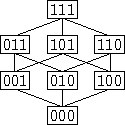
\includegraphics{img/ds/kubengraph.pdf} }
	\parbox{6.0cm}{Kubenabstand $\delta(c_1, c_2)$: Kleinste Anzahl an Kanten, die nötig sind, um $c_i$ und $c_j$ zu verbinden bzw.
	Anzahl an Literalen die in $c_1$ negiert und in $c_2$ nicht negiert vorkommen.\\
	
	\framebox{ \#Literale = \#Raumdimensionen - \#Kubusdimensionen }\\
	Max. Kubenabstand: \#Dimensionen - \#Kubusdimensionen(größter Kubus) \\
	} \\
	überdeckte Minterme: $2^{\text{Kubendimension}}$
	\subsection{(R)OBDD}
	(\textbf{R}educed) \textbf{O}rdered \textbf{B}inary \textbf{D}ecision \textbf{D}iagram\\
	\parbox{2.0cm}{ 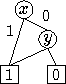
\includegraphics{img/ds/robdd.pdf} }
	\parbox{5.0cm}{ ROBDD $\rightarrow$ SOP: Alle Pfade zur 1 verodern:\\ $f = x + \overline xy$ \\ 
					ROBDD $ \ra$ POS: Alle Pfade zu 0 verodern, kompletten Term negieren, DeMorgan anwenden} \\
	


\section{Funktionale Dekomposition} % (fold)
\label{sub:Funktionale Dekomposition}
\parbox{2.7cm}{ 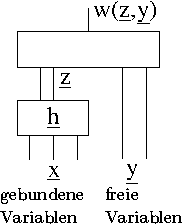
\includegraphics[width = 2.2cm]{img/ds/decomp.pdf} }
\parbox{6.0cm}{
Bei einer Funktion $f(\vec v)$ mit $n$ Eingängen und einer möglichen Aufteilung von $\vec v$ in $\vec v = \vec x$ und $\vec y$ (wobei die Aufteilung disjunkt ist), kann $f(\vec v) = f(\vec x, \vec y)$ in $g(h(\vec x), \vec y)$ zerlegt werden. \\
\\
Zerlegung sinnvol, wenn $\abs{\vec z} \le \abs{\vec x} -1$ oder $\abs{Z} \le \frac{1}{2} \abs{X}$ \\
Kompositionsfunktion: $w = g(\vec z, \vec y)$ \\
Dekompositionsfunktion: $\vec z = h(\vec x)$ \\
\\
$\ra $ Meist kann man eine günstige Aufteilung per BDD finden. }\\
\\
Verfahren:
\begin{itemize}
	\item Auswerten von $f(\vec{\hat x}, \vec y)$ und Bilder der Dekompositionsmatrix: \\
		$f = \overline x_1\overline x_2 y_1 + \overline x_1  x_2  x_3  y_1 + \overline x_1  x_2 \overline x_3  \overline y_1 \ldots$
	\item Trage die Funktionswerte in die Matrix ein
	\item Suche Spalten, die die selben Werte je $\vec y$ haben
	\item Codiere gleiche Spalten mit gleichem $z$
\end{itemize}
		\begin{tabular}{c | c | c | c | c | c | c | c | c }
			freie Variablen & \multicolumn{8}{c}{gebundene Variablen $(x_1, x_2, x_3)$}  \\
			 $(y_1, y_2)$ & 000 &  001 & 010 & 011 & 100 & 101 & 110 & 111  \\ \midrule
			00	& 0 & 0 & 1 & 0 & 1 & 1 & 1 & 1 \\
			01 & 0 & 0 & 1 & 0 & 1 & 1 & 1 & 1 \\
			10 & 1 & 1 & 0 & 1 & 0 & 0 & 0 & 0 \\
			11 & 1 & 1 & 0 & 1 & 1 & 1 & 1 & 0 \\ \midrule
			$\vec z = h(x)$ & 00 & 00 & 01 & 00 & 10 & 10 & 10 & 01
		\end{tabular}
\begin{itemize}
	\item Konstruiere die Dekompositionsfunktion \\
	$ \abs{\vec z} \le \abs{\vec x}  -1 $ bzw. $\abs{Z} \le \frac{1}{2} \abs{X}$
	\item Stelle Zuordnungstabelle auf:\\
		\begin{tabular}{ c | c | c | c }
		$\vec{\hat x_i}$ & $\vec{\hat z_i}$ & $\vec z = h(x)$ & $ g(\vec z_i, \vec y) $ \\ \midrule
		000, 001, 011 & 00 & $\overline z_1 \overline z_2 = \overline x_1 \overline x_2 + \overline x_1 x_2 x_3$ & $y_1 $\\
		010, 111 & 01 &$ \overline z_1 z_2 = \overline x_1 x_2 \overline x_3 + x_1 x_2 x_3$  & $\overline y_1$ \\
		100, 101, 110 & 10 & $z_1 \overline z_2 = x_1 \overline x_2 + x_1 x_2 \overline x_3$ & $\overline y_1 + y_2$ \\
		& 11 & & 0
		\end{tabular}
		
	\item Konstruktion der Kompositionsfunktion \\
	$\ra $ via Dekompositionsmatrix (1) / Zuordnungstabelle (2) \\
		(1) alle eingetragenen 1en $\hat =$ 1 am Ausgang \\
			$\ra$ müssen in der Kompositionsfunktion auftreten \\
		(2) $\vec{\hat z_i} \cdot g(z,y)$ stellen die Komposistionsfunktion dar \\
		\\
	$g(\vec z, \vec y) = \overline z_1 \overline z_2 y_1 + \overline z_1 z_2 \overline y_1 + z_1 \overline z_2 \overline y_1 + z_1 \overline z_2 y_1 y_2 $ = Kompositionsfunktion
	
	\item Notationen:
		$\abs{\vec x} = $ Zahl der Eingangsvariablen (gebunden) \\
		$\abs{\vec z} = $ Zahl der Dekompositionsvariablen \\
		$\abs{X} = 2^{\abs{\vec x}} =$ Zahl der möglichen Zustände aller gebundenen Variablen \\
		$\abs{Z} = 2^{\abs{\vec z}} = $ Zahl aller Dekompositionsvariablen
\end{itemize}

\subsection{Funktionale Dekomposition mit ROBDD}
Ermitteln der gebundenen bzw. freien Variablen mittels BDD: \\
\parbox{2.7cm}{ 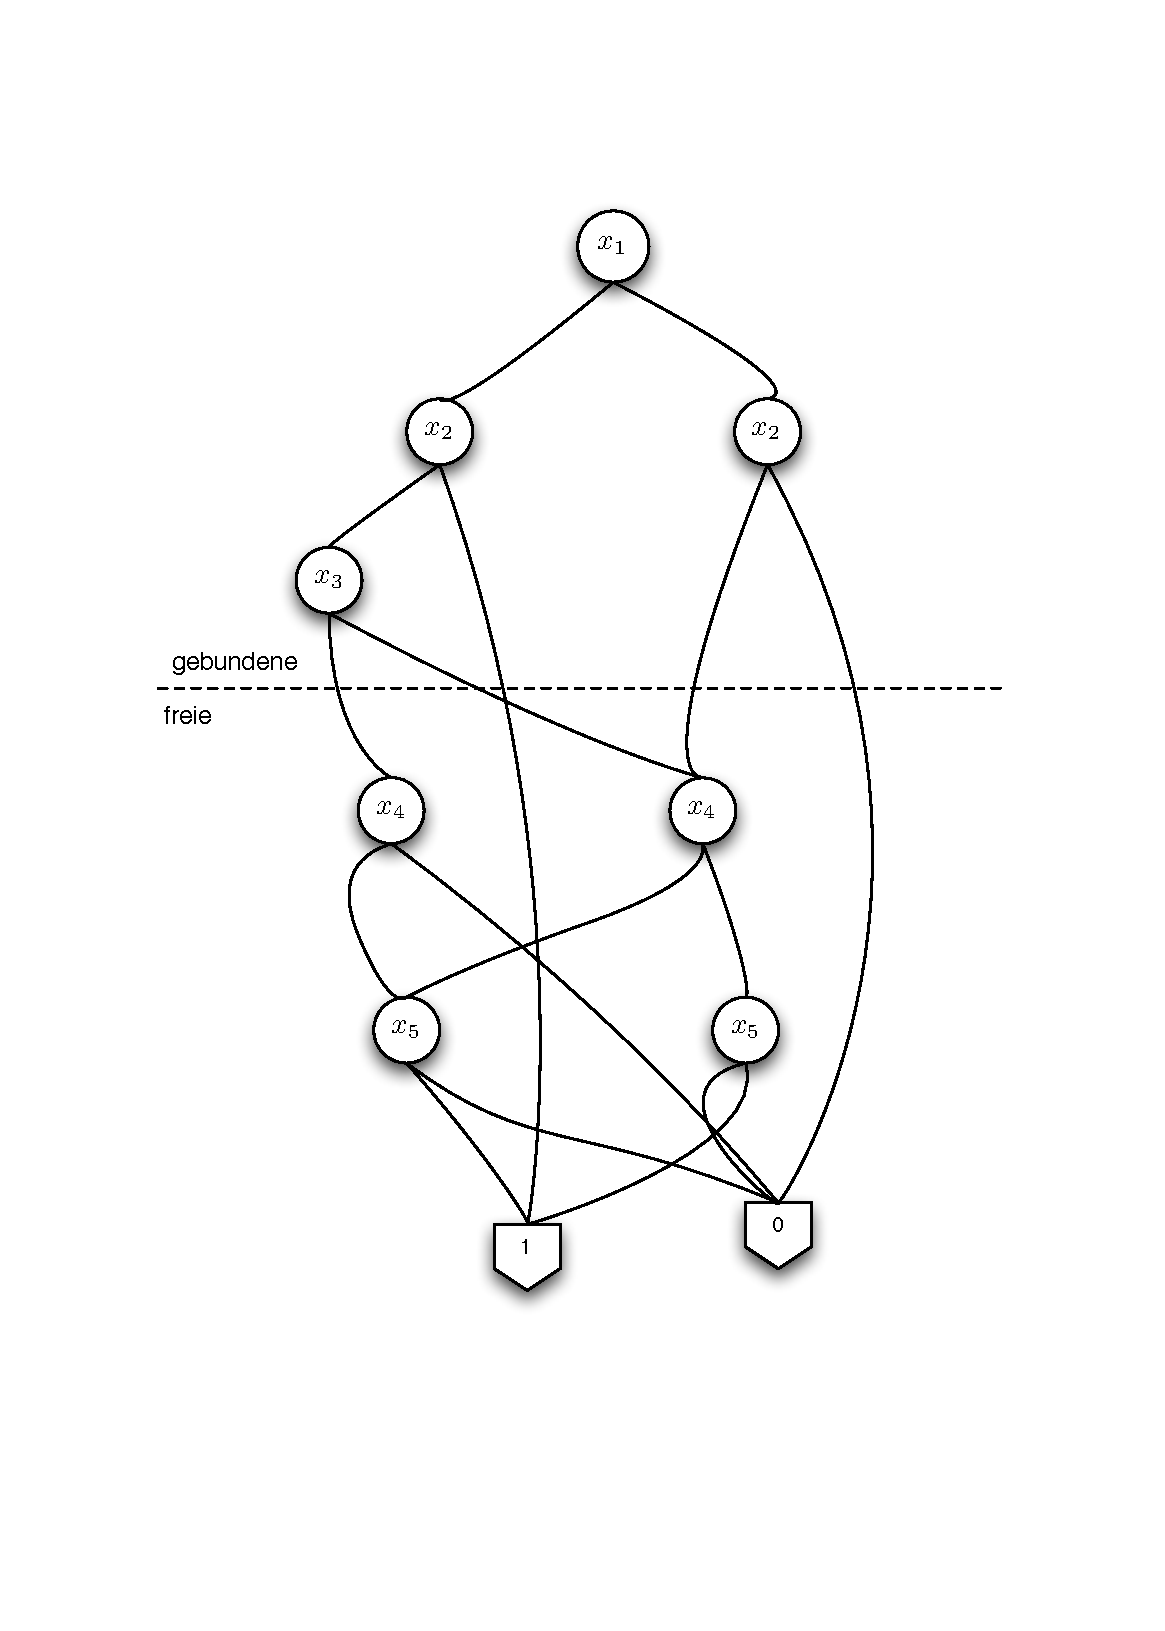
\includegraphics[width = 5cm]{img/eds/fdk.pdf} }
\paragraph{Dekompositionsbedingung} % (fold)
$\abs{\vec z} \le \abs{\vec x} - 1$ bzw. $\abs{Z} \le \frac{1}{2} \abs{X}$ \\
\begin{itemize}
	\item Nehme immer eine Ebene an:\\
	Oberhalb = gebundene Variablen \\ 
	Unterhalt = freie Variablen
	\item Zähle die Knoten, die durch die kreuzenden Äste erreicht werden (hier mit $\Delta$ bezeichnet)
	\item Auch wenn ein Knoten durch zwei oder mehrere Äste erreicht wird, darf er nur \emph{einmal} gezählt werden (im Beispiel: $\Delta = 4$)
	\item Wenn $\abs{\vec z} = \lceil \log_2 \Delta \rceil \le \abs{\vec{x}} - 1 \ra$ DK-Bed. erfüllt
	\item Pfade zur 1 ergeben Dekompositionsfunktion ( gebundene Variablen \ra freie Variablen \ra 1)
\end{itemize}
Zuordnungstabelle:\\
\begin{tabular}{l|cc|l}
geb. Variablen & $z_1$ & $z_2$ & freie Variablen \\ \midrule
111 & 0 & 0 & $x_4 x_5$ \\
110, 010, 011 & 0 & 1 & $x_4 x_5 + \ol x_4 \ol x_5$ \\
101, 100 & 1 & 0 & 1 \\
& 1&1& \\
\end{tabular}
% subsection Funktionale Dekomposition (end)

\subsection{Heuristische Minimierung}
Kofaktorbildung: Setze alle $x_i = 1$ und alle $\overline x_i = 0$ \\
z.B. $f = x\overline y + \overline x yw + x w \Ra f_x = \overline y + w$


\subsubsection{Kubenentfernung (remove)}
\begin{itemize}
	\item $h = f \setminus c$ ($f$ ohne den zu entfernenden Kubus) \\
	z.B. $ f = \overline x y z+ x y z + \overline x  yz \Ra \text{ für } c = \overline x y z \Ra h =  xyz + \overline x y z$ \\
	$h_{\ol xyz} = 1 + 0 = 1 \Ra$ entfernbar
	\item Bildung des Kofaktors $h_c$
	\item Wenn $h_c = 1 \Ra c$ ist entfernbar
\end{itemize}
2 Kuben gemeinsam entfernen: teste 2. Kubus \textbf{nachdem} der 1. entfernt wurde.
\subsubsection{Literalentfernung (expand)}

\begin{itemize}
	\item Aufstellen von $h = \eset{f \setminus c_l \cdot l}$ \\
	z.B. $ f = \overline x y + x y z + \overline x \cdot \overline y \cdot \overline z$ (entferne $x$: d.h. $l = x$ und $c_l = yz$) \\ 
	$h = \overline x y  + \overline x \cdot \overline y \cdot \overline z$
	\item Wenn $h_{c_l \cdot \overline l} = 1$ ist das Literal entfernbar \\
	z.B. $h_{c_l \cdot \overline l} = (\overline x y  + \overline x \cdot \overline y \cdot \overline z)_{\overline x y z} = 1$
\end{itemize}

\subsubsection{Literal hinzufügen (reduce)}
Kann man $l$ zu $c$ hinzufügen ohne $f$ zu verändern? \\
$f = c + h \overset{?}{=} c \cdot l + h$
\\ Zulässigkeitsbedingung: $c \cdot \overline l \subseteq h$ \\
z.B. $f = xy + \overline x y z + xz$ (füge $l = \overline z$ hinzu) \\
Ist $xyz \subseteq \overline x yz + xz$? \\
Ja $\Ra f^* = xy \overline z + \overline x yz + xz$

Gemeinsame Literalentfernung: Prüfe 2. Literal nachdem 1. Literal entfernt wurde.\\

\subsection{Strukturanalyse}
Tautologie: $f_{x_i} = 1 \ \land \ f_{\overline x_i} = 1 \quad \Rightarrow f=1$\\
Monoton steigend in $x_i$: \boxed{ f_{\overline x_i} \subseteq f_{x_i}} dann gilt auch $f_{\ol x_i} = 1 \ \Ra\ f = 1$\\
Monoton fallend in $x_i$: \boxed{ f_{x_i} \subseteq f_{\overline x_i} } dann gilt auch $f_{x_i} = 1 \ \Ra\ f = 1$\\
Beispiel: \\
$f = yz + xz + \n y z + \n y \n z + y \n z \Ra$ monoton steigend in $x$ \\
$f(x,y,z) = x \; \varphi (z) + h(y,z) \Ra $ Prüfe $h$ auf Tautologie

\section{Nützliches Wissen}
\subsection{Mehrfachimplikanten}
Sind gleiche Implikanten in mehreren verschiedenen Funktionen vorhanden? \\ 
Prüfe  $f_1 \cap f_2 $ auf Mehrfachimplikanten: $f_1 \cdot f_2 = ?$ \\
Nutzung von Mehrfachimplikanten ist sinnvoll wenn die Gesamtliteralzahl beider SOPs kleiner ist als ohne Verwendung von Mehrfachimplikanten.

\subsection{VollSOP erstellen} % (fold)
\label{sub:VollSOP erstellen}
Benutze die Resolventenmethode um alle Resolventen zu erzeugen und so aus der MinSOP eine VollSOP zu erstellen.
% subsection VollSOP erstellen (end)

\section{Automaten}
sind abstrakte Maschinen mit $r$ Zuständen $S_i \in S$ , die auf sequentielle Eingangssignale $X_j \in I = \mathbb B^n$ mit Ausgangssignalen $Y_l\in O = \mathbb B^m$ und Zustandsänderungen reagiern.\\
\begin{tabular}{ll}
	Startzustand & $S^0 \in S$ \\
	Zustandsfkt. & $\delta : S \times I \rightarrow S,\ S_k \mapsto \delta(S_i , X_j)$ \\
	Ausgangsfkt. & $\lambda : S \times I \rightarrow O,\ Y_l \mapsto \lambda(S_i , X_j)$ \\
	ZA-fkt. & $\mu : S \times I \rightarrow S \times O,\ (S_k, Y_l) \mapsto \mu(S_i , X_j)$ \\
\end{tabular}\\
\\
\paragraph{$k$-Äquivalenz $S_i \stackrel{k}{\sim} S_j$} 
Für eine Eingangssequenz der Länge $k$ sind bei $S_i$ und $S_j$ die Ausgaben gleich und die Zustandsübergänge gleich bzw. $k-1$ Äquivalent.\\
\paragraph{Totale Äquivalenz $S_i \sim S_j$} falls für alle Einganssequenzen die Ausgaben und die Zustandsübergänge äquivalent sind. \\ $\ra$ Zeige: es lassen sich keine weiteren Äquivalenzklassen bilden.\\


\section{Karnaugh- Diagramm} % (fold)
	Zyklische Gray-Codierung: 2dim:$00,01,11,10$ 3dim:$000,001,011,010,110,111,101,100$
	
\begin{tabular}{l | c | c |  c | r}
$_z\!\!\diagdown \!\!^{xy}$ & 00 	& 	01	&	11 	&	10	 	\\ \midrule
0		&	1 \cellcolor{gray}	&	0	&	0	&	0		\\	
1		&	X \cellcolor{gray}	&	1 \cellcolor{lightgray}	&	1 \cellcolor{lightgray}	&	0		\\	
\end{tabular}
Gleiche Zellen zusammenfassen: z.B. $\overline x \overline y + y \cdot z$\\
Don't Care Werte ausnutzen!\\
% section Karnaugh- Diagramm (end)


\section{Resolventenmethode} % (fold)
\label{sec:Resolventenmethode}
	Ziel: alle Primimplikanten \\
	
	Wende folgende Gesetze an: \\
	Absorptionsgesetz: $a + ab = a$ \\
	allgemeines Resolutionsgesetz: $x \cdot a + \overline x \cdot b = x \cdot a + \overline x \cdot b + ab$ \\
	\\
	Anwendung mit Schichtenalgorithmus
	\begin{enumerate}
		\item schreibe die Funktion $f$ in die 0. Schicht
		\item bilde \textbf{alle möglichen} Resolventen aus der 0. Schicht und schreibe sie in die nächste Schicht als ODER Verknüpfungen (Resolventen zu $f$ "hinzufügen")
		\item überprüfe ob Resolventen aus der 1. Schicht Kuben aus Schicht 0 überdecken(Absorbtion) und streiche diese Kuben aus Schicht 0
		\item Schicht i besteht aus den möglichen Resolventen von Schicht 0 bis $(i-1)$. Abgestrichene Kuben aus vorherigen Schichten brauchen \textbf{nicht} mehr beachtet werden.
		\item Sobald in der i-ten Schicht +1 steht oder keine weiteren Resolventen gebildet werden können, ist man fertig. 
		$\Ra $ alle nicht ausgestrichenen Terme bilden die VollSOP
	\end{enumerate}
	
	\begin{tabular}{l | r}
	$f(x_1, \ldots, x_n)$ & Schicht \\ \midrule
	$x \cdot w + \overline x \cdot w + x \cdot y \cdot w \cdot \overline z + \overline x \cdot y \cdot w \cdot \overline z + \overline y \cdot w \cdot \overline z $& $0$ \\
	$+ w + y \cdot w \cdot \overline z$ & $1$ \\
	$+ w \cdot \overline z $ & $2$ \\
	$+ w$ &$ 3$
	\end{tabular}
% section Resolventenmethode (end)

\section{Laufzeit}

	\subsection{Laufzeitabhängige Effekte}
	\begin{itemize}
		\item \emph{Race}, "'Wettlauf"' zweier Signalwertänderungen vor einem gemeinsamen Gatter\\
		\item \emph{Hazard / Spike / Glitch}, Stelle des Signalwertverlaufes, die wegen der Laufzeitverzögrung nicht den Erwartungen entspricht\\
	\end{itemize}

	\subsection{Simulation}
	\pbox{4cm}{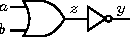
\includegraphics[scale = 0.8]{img/ds/laufzeit.pdf}}
	\pbox{9cm}{ $\tau_{OR}=2$ und $\tau_{NOT}=1$ Eingangsbelegung $a=0$,$b=0$ \\Eingangsereignis (b,'1',0, 2) }\\
	Auswertung erfolgt durch eine Tabelle:\\
 	\begin{tabular}{l|cccc|l|l}
		t& a &b &z &y& ausgewertete Elemente & neue Ereignisse\\ \midrule
		0& '0' & '0' & '1'& '0' & init & (b,'1',0, 2) \\
		2& & '1' & & & OR & (z,'1',2,4) \\
		4& & & '1' & & NOT & (y,'0',4,5)\\
		5& & & & '0' &  & \\
	\end{tabular}
	\\
	Ereignis: (betroffenes Signal, neuer Signalwert, $t$, $t+\tau$)

	\subsection{Delay}
	\begin{itemize}
		\item transport delay: Verzögerung um $\tau_{pd} $
		\item inertial delay: Verzögerung um $\tau_{pd}$ und Impulse die kleiner als $\tau_{pd}$ sind werden ignoriert
	\end{itemize}


	\subsection{VHDL- VHSIC Hardware Description Language}
	\begin{tabular}{ll}
	\texttt{ENTITY} Bausteinname  \texttt{IS}	& //Definiert die Schnittstelle einer Logik\\
	\texttt{PORT} (Schnittstellenliste) & //Definiert Ein- und Ausgänge\\
	\\
	\texttt{ARCHITECTURE} Rumpfname \texttt{OF} Bausteinname \texttt{IS} & //Beschreibt den internen Aufbau\\
	\texttt{PROCESS} (Signalliste) & // Alle Processes laufen nebeneinander ab\\
	\texttt{COMPONENT} Gattername & // Beschreibt eine interne Komponente\\
	\end{tabular}

\section{Testverfahren}
Mit wenig Fragen viel Information erhalten. Signal muss beobachtbar und einstellbar sein!\\

	\subsection{Begriffe}
	Fehlergruppe $F_\nu = \iset{f_\mu \in F}{t_\nu R f_\mu}$: Menge aller Fehler die vom Test $t_\nu$ erkannt werden.\\
	Fehleranzahl = $2 \cdot$ Signalanzahl = $2 (\text{Eingänge} + \text{Interne Signale} + \text{Ausgänge})$\\
	Testgruppe $T_\mu = \iset{t_\nu \in T}{t_\nu R f_\mu}$ ist die Menge aller Tests die den Fehler $f_\mu$ erkennen.\\

	Zwei einzelne Fehler sind nicht unterscheidbar, wenn sie immer gemeinsam von einem Test entdeckt werden.\\ 

	\subsection{Bullshit-Differenz $y_z$}
	Ziel: schnelles finden von Testbedingungen für $f = y(z(\vec x))$\\
	\\
	\boxed{ y_z = y(z,\vec x) \oplus y(\overline z, \vec x) } \ $\mathrel{\widehat{=}} y(z = 1) \oplus y(z=0)$\\
	
	\subsubsection{Rechenregeln}
	\begin{tabular}{ll}
		$y_x = 0$ \ falls $y \ne f(x)$ & $(z \cdot w)_x = z \cdot w_x \oplus z_x \cdot w \oplus z_x \cdot w_x$\\ 
		$y_y =1$ & $(z + w)_x = \overline z \cdot w_x \oplus z_x \cdot \overline w \oplus z_x \cdot w_x$\\
		$(\overline y)_x = y_x$ & $y_x = y_z \cdot z_x$ \ falls $y = y(z(x))$\\
		$(z \oplus w)_x = z_x \oplus w_x$ & $(y_z)_w = (y_w)_y$\\
	\end{tabular}
	\subsubsection{AND $\rightarrow$ XOR $(+,\overline x)$}
	Vorgehen:
	\begin{enumerate}\itemsep-2pt
		\item Negation über konjunkte Terme entfernen: DeMorgan $\ol {xy} = \ol x + \ol y)$
		\item Negation über disjunkte Terme entfernen: $\ol x = x \oplus 1)$
		\item "$+$"\ entfernen $x + y = x \oplus y \oplus xy$\\
	\end{enumerate}
	Test für $\begin{cases} a/0: a\cdot y_a \stackrel{!}= 1\\
	a/1: \overline a\cdot y_a \stackrel{!}= 1
	\end{cases}$
	$\Rightarrow$ Testmuster finden.
	
	\subsubsection{XOR-Regeln}
	\begin{tabular}{l l l}
				$ x \oplus y = \overline x \cdot y + x \cdot \overline y$ & $x + y = x \cdot y \oplus x \oplus y$ \\
				$x \oplus y = (x+y) \cdot (\ol x + \ol y)$ & $x \cdot y = x \oplus y \oplus (x+y)$\\
				$ x \cdot (y \oplus z) = x \cdot y \oplus x \cdot z$ & $ \overline x = x \oplus 1$ \\
				$x \oplus x = 0$ & $x \oplus 0 = x$ \\
				$(x+y)\oplus y = x \cdot \ol y$ & $x \ol y + y z = x\ol y \oplus y z$\\
		\end{tabular}
		
	\subsubsection{Schaltnetze}
	\parbox{3.6cm}{
	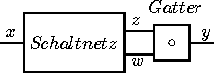
\includegraphics{img/ds/schaltnetz.pdf} }
	\parbox{5.0cm}{ 
	\begin{tabular}{ll}
	& $y = z \circ w$ \\
	Lokal: & $y_z = (\ol z \circ w) \oplus(z \circ w)$\\
	& $y_w = (z \circ \ol w) \oplus(z \circ w)$\\ \midrule
	Global: & $y_x = [(z \oplus z_x) \circ (w \oplus w_x)] \oplus [z \circ w]$
	\end{tabular}
	}\\[0.5em]
	\boxed{y_x = y_z  z_x  \ol w_x + y_w  w_x \ol z_x + z_x  w_x \cdot [\ol z \circ \ol w \oplus z \circ w]}\\	
	$\circ =$ XOR/XNOR $\  \Ra \ [\ol z \circ \ol w \oplus z \circ w] = 0$ \\ 
	$\circ =$ AND/NAND/OR/NOR $\ \Ra \ [\ol z \circ \ol w \oplus z \circ w] = \ol{z \oplus w}$\\
	\\
	Schaltnetz mit Rekonvergenzmasche (4 Fälle):\\
	\begin{tabular}{lll}
		1. & $y_z  z_x  \ol w_x = 1$ & $\Ra \ $ Einfachpfadsensibilisierung: $x$---$z$---$y$\\
		2. & $y_w  w_x \ol z_x = 1$ & $\Ra \ $ Einfachpfadsensibilisierung: $x$---$w$---$y$\\	
		3. & $z_x  w_x \cdot [\ol z \circ \ol w \oplus z \circ w] = 1$ & $\Ra \ $ Mehrfachpfadsensibilisierung\\[0.2em]
		4. & $z_x  w_x \cdot \ol{ [\ol z \circ \ol w \oplus z \circ w] } = 1$ & $\Ra \ $ Selbstmaskierung\\
	\end{tabular}
	\\[1em]
	Schaltnetz mit Baumstruktur: \\
	keine Mehrfachpfadsensibilisierung oder Selbstmaskierung!\\
	$y_x = y_z \cdot z_x$ (Kettenregel für $x$---$u$---$z$---$y$)\\
	
	\subsection{Fehlersimulation}
	Gegeben: Testmuster \quad	Gesucht: getestete Fehler.\\ \\
	\paragraph{Achtung} Teste immer nur für eine spezielle Belegung 
	\paragraph{Begriffe} 
	Fanout-Stamm: Verzweigungspunkt \quad
	Vereinigungspunkt: Rekonvergenzpunkt \\
	
	
	\subsubsection{Fehlerbaumkonstruktion für gegebenes Testmuster}
	\begin{enumerate}
	\item Alle Signalwerte der Schaltung für gegebenes Testmuster bestimmen
	\item Durch die Simmulation die Beobachtbarkeit der Fanout-Stämme bestimmen.
	\item Schaltung an Fanout-Stämmen gedanklich auftrennen. (In Fanout-Freie Zonen zerlegen)
	\item Fehlerbaumkonstruktion in den Bäumen(FF-Zonen) vom Ausgang in Richtung Eingänge auf Basis der lokalen Sensitivitäten (mit $\bullet$ markieren).
	\item Aus Fehlerbaum Menge der beobachtbaren Signale $S^0$ (sensitiver Pfad zum Ausgang) und Menge der getesteten Fehler $F_t$ durch Einstellbarkeit (sensitiver Pfad zum Eingang) angeben.
	z.B. $S^\circ =\{ a, b, b_2, y \}$ \quad $F_t = \{ a/1 , b / 0 , b_2/0 y / 1 \}$\\
	\end{enumerate}


	

	\subsection{Deterministische Testmustergenerierung. D-Algorithmus}
	Zahl aller Fehlerpfade: $2^n -1$ für $n =$ Zahl der Einfachfehlerpfade\\ \\
	Findet für jeden stuck-at Fehler einen Test, falls möglich.\\
	5-wertige Logik:\\
	\begin{tabular}{ll}
		0 & Boolsche 0 \\
		1 & Boolsche 1\\
		$X$ & undefined \\
		$D$ & 1 falls fehlerfrei, 0 falls fehlerhaft (teste stuck-at 0)\\
		$\overline D$ & 0 falls fehlerfrei, 1 falls fehlerhaft (teste stuck-at 1)\\
	\end{tabular}
	
	Lokale Implikation:
	\begin{tabular}{ll}
	Vorwärtsimlikation & Rückwärtsimlikation\\
	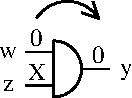
\includegraphics[scale = 0.8]{img/ds/vorimplikation.pdf} & 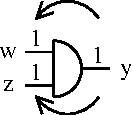
\includegraphics[scale = 0.7]{img/ds/backimplication.pdf}\\%	\includegraphics{img/ds/vorimplikaiton.pdf} & \includegraphics{img/ds/rückimplikaiton.pdf} \\
	\end{tabular}
	\\
	globale Implikation: mehr als 1 Gatter zwischen Testsignal und implizierten Signal:\\
	\boxed{ A \Ra B \ \Leftrightarrow\  \ol B \Ra \ol A}\\
	Lernkriterium (für $y=z(x)$): $y_{z_1} \cdot y_{z_2} \stackrel{!}= 1$\\

	Vorgehen (z.B für Test $x_1/0$):\\
	$F:$ Fehlertestsignal ($x_1 = D$)\\
	$S:$ Sensibilisierung ($x_2 = 1$)\\
	$I:$ Impliaktion ($y = \ol D$)\\
	$O:$ Optionale Pfade (z.B bei XOR)\\
	\\
	Ist Ausgang $0$ bzw. 1 $\Ra$ Fehler nicht testbar.\\
	Ist Ausgang $D$ bzw. $\ol D\ \Ra$ Fehler testbar.\\

	\subsection{Einstellbarkeit}
	\parbox{2.5cm}{ \framebox{$C_0 + C_1 = 1$} }
	\parbox{4.0cm}{
		$C_0$: Nulleinstellbarkeit $ 0 \le C_0 \le 1 $ Wahrscheinlichkeit das ein Testvektor zur 0 führt\\
		$C_1$: Einseinstellbarkeit $ 0 \le C_1 \le 1 $
	}\\
	ohne Vorgabe für Eingangsvariable~x: $C_0(x)=0,5$ und $C_1(x)=0,5$\\
	Beachte: Je nach Gatter sind besimmte Einstellbarkeiten schneller zu berechnen! (siehe Tabelle)\\
	\begin{tabular}{l|c|l}
	Gatter & Einstellbarkeit (Ausgang) & Berechnung\\ \midrule
	AND & $C_1$ & $C_1(x_1) \cdot C_1(x_2)$ \\
	NAND & $ C_0$ & $C_1(x_1) \cdot C_1(x_2)$ \\
	OR & $C_0$ & $C_0(x_1) \cdot C_0(x_2)$ \\
	NOR & $C_1$ & $C_0(x_1) \cdot C_0(x_2)$ \\
	XOR & $C_1$ & $C_0(x_1) \cdot C_1(x_2) + C_1(x_1) \cdot C_0(x_2)$ \\
	NOT & $C_1$ & $C_0(x)$ \\
	\end{tabular}
	\newline Wichtig: Nur bei Baumstruktur exakt.\\

	\subsection{Schaltwerke}
	\begin{tabular}{ll}
		Eingangsvariable 			& 		$\ma X$	\\
		Testpunkte 					& 		$\ma Y$	\\
		nächste Schaltwerkszustände & 		$\ma Z$	\\
		Schaltwerkszustände 		&		$\ma S$	\\
	\end{tabular}									\\
	
	Es gilt: $\vec s^t = \vec z^{t-1}$ \qquad $t:$ $t$-te Taktperiode.\\
	\\
	Verbesserung der Einstellbarkeit und Beobachtbarkeit durch Zusatzlogik:\\
	Zusätzlicher Testeingang: Mehr Platzbedarf, mehr Leistungsaufnahmen.\\
	Zusätzlicher Ausgang: Zusätzlicher Pin, langsameres Signal.\\
	
\section{Auch wichtig}
\parbox{1.2cm}{
 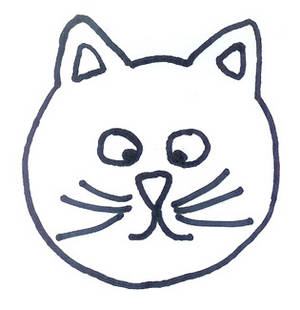
\includegraphics[width=1cm]{img/cat.jpg}
 }
 \parbox{3cm}{
\emph{Schrödingers Katze}
}
\end{multicols}


% Dokumentende
% ======================================================================
\end{document}
